\textbf{
    (El problema del escape) Una malla de $n x n$ es una gráfica compuesta por $n$ filas y
    $n$  columnas de vértices cómo se muestra en la figura 1. Denotamos el vértice en la 
    i-ésima fila y j-ésima columna como $(i, j)$. Todos los vértices en una malla tienen 
    exactamente cuatro vecinos, excepto aquellos en la frontera, que son los vertices 
    $(i,j)$, donde $i = 1, n$ o $j = 1, n$.
}

\textbf{
    Dados $m \leq n^2$ vértices de arranque $(x_1,y_1),(x_2,y_2), \dots ,(x_m,y_m)$ en la 
    malla, el problema del escape es decidir si existen $m$ trayectorias ajenas por vértices
    que conecten a cada vértice de arranque con algún vértice en la frontera (distintos).
}\vspace{.2cm}

\begin{figure}[H]
    \centering
        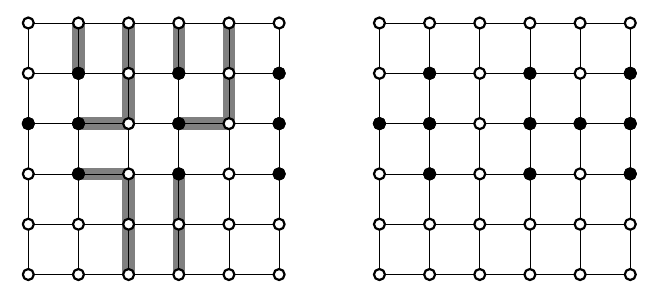
\includegraphics[height=3.3cm]{src/Img/8.png}
        \caption{Izquierda malla con escapatoria. Derecha: una sin escapatoria}
\end{figure}
